%**************************************************************
% Lab 06: Counter
%**************************************************************
\chapter{Counters}

Counters are perhaps the most commonly-used circuits in electronic devices. They are found in virtually all electronics systems, from the simplest embedded computers to massive mainframes. Counters are designed to cycle through a specific predefined sequence of binary numbers when an input pulse is applied. Typically, counters simply count up or down from given start and end numbers, but they can be designed to produce unique output patterns for special uses. 

Counters, though, are used for more than simple counting. They can measure time so devices like alarm clocks and watches include counters. They are used as frequency dividers so a fast input frequency can be output at a slower rate. In devices with memory they are used to increment memory addresses as a program steps through some process. They can activate a series of subcircuits in sequence as part of a complex process. They are, in short, one of the most important workhorses of the digital logic world.

\section{Purpose}

This lab has two goals: 

\begin{enumerate}
	\item Develop several different common counters using \textit{D} flip-flops. Because there are two main families of counters, asynchronous and synchronous, this lab includes examples of both. 
	\item Introduce the \textit{Logisim-evolution} chronogram feature that generates a timing diagram as a sequential circuit functions. 
\end{enumerate}

\section{Procedure}

\subsection{Asynchronous Up Counter}

A counter is built from a series of flip-flops and where the output from each flip-flop is combined to create the counter output, the trigger the next flip-flop, or both. Each flip-flop is considered a ``stage'' of the counter. A counter is triggered by a clock signal that is typically supplied by a timer with a regularly-recurring pattern of high/low levels, but it can also be triggered by an event of some sort, like the completion of a process.

\marginpar{In all Counter circuits in this manual flip-flop U0 provides the Least Significant Bit to the output and U3 provides the Most Significant Bit.}One of the simplest counters is illustrated in Figure \ref{fig:06-01}. This is an asynchronous four-stage up counter. A counter is is considered ``asynchronous'' if the input clock signal is applied to only the first stage and then that signal ripples through each flip-flop in turn. Thus, an asynchronous counter is frequently called a ``ripple'' counter.

\begin{figure}[H]
	\centering
	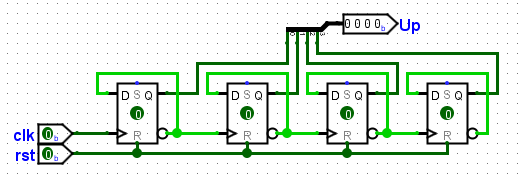
\includegraphics[width=\maxwidth{.95\linewidth}]{gfx/06-01}
	\caption{Asynchronous Up Counter}
	\label{fig:06-01}
\end{figure}

The following list describes the operation of the counter in Figure \ref{fig:06-01}:

\begin{description}
	\item [Reset is Activated] All flip-flops are reset so \textit{Q} is low and \textit{Q'} is high.

	%%%%%%%%%%%%%%%
	\item [Tick 1] \textit{U0} clocked: \textit{Q0} \textuparrow \: \textemdash \: \textit{Q'0} \textdownarrow

	%%%%%%%%%%%%%%%
	\item [Tick 2] \textit{U0} clocked: \textit{Q0} \textdownarrow \: \textemdash \: \textit{Q'0} \textuparrow
	
	\hspace{14pt}\textit{U1} clocked: \textit{Q1} \textuparrow \: \textemdash \: \textit{Q'1} \textdownarrow
	
	%%%%%%%%%%%%%%%
	\item [Tick 3] \textit{U0} clocked: \textit{Q0} \textuparrow \: \textemdash \: \textit{Q'0} \textdownarrow

	%%%%%%%%%%%%%%%
	\item [Tick 4] \textit{U0} clocked: \textit{Q0} \textdownarrow \: \textemdash \: \textit{Q'0} \textuparrow

	\hspace{14pt}\textit{U1} clocked: \textit{Q1} \textdownarrow \: \textemdash \: \textit{Q'1} \textuparrow

	\hspace{14pt}\textit{U2} clocked: \textit{Q2} \textuparrow \: \textemdash \: \textit{Q'2} \textdownarrow

	%%%%%%%%%%%%%%%
	\item [Tick 5] \textit{U0} clocked: \textit{Q0} \textuparrow \: \textemdash \: \textit{Q'0} \textdownarrow

	%%%%%%%%%%%%%%%
	\item [Tick 6] \textit{U0} clocked: \textit{Q0} \textdownarrow \: \textemdash \: \textit{Q'0} \textuparrow

	\hspace{14pt}\textit{U1} clocked: \textit{Q1} \textuparrow \: \textemdash \: \textit{Q'1} \textdownarrow
	
	%%%%%%%%%%%%%%%
	\item [Tick 7] \textit{U0} clocked: \textit{Q0} \textuparrow \: \textemdash \: \textit{Q'0} \textdownarrow

	%%%%%%%%%%%%%%%
	\item [Tick 8] \textit{U0} clocked: \textit{Q0} \textdownarrow \: \textemdash \: \textit{Q'0} \textuparrow

	\hspace{14pt}\textit{U1} clocked: \textit{Q1} \textdownarrow \: \textemdash \: \textit{Q'1} \textuparrow
	
	\hspace{14pt}\textit{U2} clocked: \textit{Q2} \textdownarrow \: \textemdash \: \textit{Q'2} \textuparrow

	\hspace{14pt}\textit{U3} clocked: \textit{Q3} \textuparrow \: \textemdash \: \textit{Q'3} \textdownarrow

\end{description}

As the clock continues the counter would cycle through the binary values 1001 - 1111. The following table lists the \textit{Up} counter output as indicated by the \textit{Q} values at each tick listed above.

\begin{table}[H]
	\sffamily
	\newcommand{\head}[1]{\textcolor{white}{\textbf{#1}}}		
	\begin{center}
		\rowcolors{2}{gray!10}{white} % Color every other line a light gray
		\begin{tabular}{cc} 
			\rowcolor{black!75}
			\head{Tick} & \head{Output} \\
			Reset & 0000 \\
			1 & 0001 \\
			2 & 0010 \\
			3 & 0011 \\
			4 & 0100 \\
			5 & 0101 \\
			6 & 0110 \\
			7 & 0111 \\
			8 & 1000
		\end{tabular}
	\end{center}
	\caption{Up Counter Output}
	\label{tab0601}
\end{table}

\subsection{Asynchronous Down Counter}

The asynchronous down counter illustrated in Figure \ref{fig:06-02} is very similar to the up counter in Figure \ref{fig:06-01} except the stages are triggered from the \textit{Q} output of the preceding stage rather than \textit{Q'} and the \textit{Reset} signal is applied to the flip-flop \textit{S} input rather than \textit{R}.

\begin{figure}[H]
	\centering
	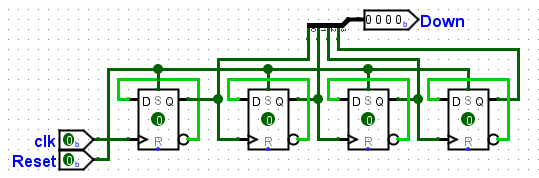
\includegraphics[width=\maxwidth{.95\linewidth}]{gfx/06-02}
	\caption{Asynchronous Down Counter}
	\label{fig:06-02}
\end{figure}

The following list describes the operation of the counter in Figure \ref{fig:06-02}:

\begin{description}
	\item [Reset is activated] All flip-flops are set so \textit{Q} is high and \textit{Q'} is low.
	
	\item [Tick 1] \textit{U0} clocked: \textit{Q0} \textdownarrow \: \textemdash \: \textit{Q'0} \textuparrow

	%%%%%%%%%%%%%%%
	\item [Tick 2] \textit{U0} clocked: \textit{Q0} \textuparrow \: \textemdash \: \textit{Q'0} \textdownarrow
	
	\hspace{14pt}\textit{U1} clocked: \textit{Q1} \textdownarrow \: \textemdash \: \textit{Q'1} \textuparrow
	
	%%%%%%%%%%%%%%%
	\item [Tick 3] \textit{U0} clocked: \textit{Q0} \textdownarrow \: \textemdash \: \textit{Q'0} \textuparrow

	%%%%%%%%%%%%%%%
	\item [Tick 4] \textit{U0} clocked: \textit{Q0} \textuparrow \: \textemdash \: \textit{Q'0} \textdownarrow
	
	\hspace{14pt}\textit{U1} clocked: \textit{Q1} \textuparrow \: \textemdash \: \textit{Q'1} \textdownarrow
	
	\hspace{14pt}\textit{U2} clocked: \textit{Q2} \textdownarrow \: \textemdash \: \textit{Q'2} \textuparrow

	%%%%%%%%%%%%%%%
	\item [Tick 5] \textit{U0} clocked: \textit{Q0} \textdownarrow \: \textemdash \: \textit{Q'0} \textuparrow

	%%%%%%%%%%%%%%%	
	\item [Tick 6] \textit{U0} clocked: \textit{Q0} \textuparrow \: \textemdash \: \textit{Q'0} \textdownarrow
	
	\hspace{14pt}\textit{U1} clocked: \textit{Q1} \textdownarrow \: \textemdash \: \textit{Q'1} \textuparrow

	%%%%%%%%%%%%%%%
	\item [Tick 7] \textit{U0} clocked: \textit{Q0} \textdownarrow \: \textemdash \: \textit{Q'0} \textuparrow

	%%%%%%%%%%%%%%%
	\item [Tick 8] \textit{U0} clocked: \textit{Q0} \textuparrow \: \textemdash \: \textit{Q'0} \textdownarrow
	
	\hspace{14pt}\textit{U1} clocked: \textit{Q1} \textuparrow \: \textemdash \: \textit{Q'1} \textdownarrow
	
	\hspace{14pt}\textit{U2} clocked: \textit{Q2} \textuparrow \: \textemdash \: \textit{Q'2} \textdownarrow
	
	\hspace{14pt}\textit{U3} clocked: \textit{Q3} \textdownarrow \: \textemdash \: \textit{Q'3} \textuparrow
	
\end{description}

As the clock continues the counter would cycle through the binary values 0110 - 0000. The following table lists the \textit{Down} counter output as indicated by the \textit{Q} values at each tick listed above.

\begin{table}[H]
	\sffamily
	\newcommand{\head}[1]{\textcolor{white}{\textbf{#1}}}		
	\begin{center}
		\rowcolors{2}{gray!10}{white} % Color every other line a light gray
		\begin{tabular}{cc} 
			\rowcolor{black!75}
			\head{Tick} & \head{Output} \\
			Reset & 1111 \\
			1 & 1110 \\
			2 & 1101 \\
			3 & 1100 \\
			4 & 1011 \\
			5 & 1010 \\
			6 & 1001 \\
			7 & 1000 \\
			8 & 0111
		\end{tabular}
	\end{center}
	\caption{Down Counter Output}
	\label{tab0602}
\end{table}


\subsection{Asynchronous Decade Counter}

Binary counters, like those considered in Figure \ref{fig:06-01} and Figure \ref{fig:06-02} are only able to count to a value that is a power of two but it is often necessary to build a counter that stops at some other value. These types of counters are called ``mod'' counters (short for ``modulus'') since they count up to a preset value then reset and start over, like modulus math. One of the most common mod counters is one that has ten states (it counts from zero to nine) and then resets, and that type of counter is referred to as a decade counter. Decade counters are found in any application that has to count in decimal for easy human interpretation.

The logic of a  mod counter is to add an \texttt{AND} gate on the outputs such that the output of the \texttt{AND} gate is high when the flip-flop outputs equal the mod number. For example, the \texttt{AND} gate for a decade counter would go high when the count reaches ten and that signal would immediately reset the counter back to zero.

\begin{figure}[H]
	\centering
	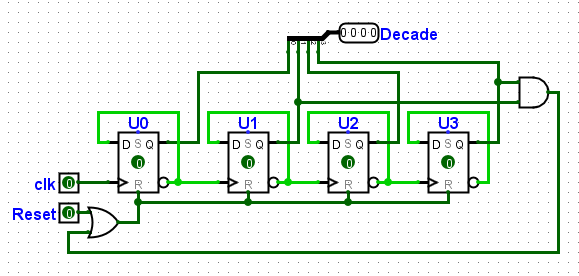
\includegraphics[width=\maxwidth{.95\linewidth}]{gfx/06-03}
	\caption{Asynchronous Decade Counter}
	\label{fig:06-03}
\end{figure}

The following list describes the operation of the counter in Figure \ref{fig:06-03}:

\begin{description}
	\item [Reset is activated] All flip-flops are reset so \textit{Q} is low and \textit{Q'} is high.
	
	%%%%%%%%%%%%%%%
	\item [Tick 1] \textit{U0} clocked: \textit{Q0} \textuparrow \: \textemdash \: \textit{Q'0} \textdownarrow
	
	%%%%%%%%%%%%%%%
	\item [Tick 2] \textit{U0} clocked: \textit{Q0} \textdownarrow \: \textemdash \: \textit{Q'0} \textuparrow
	
	\hspace{14pt}\textit{U1} clocked: \textit{Q1} \textuparrow \: \textemdash \: \textit{Q'1} \textdownarrow
	
	%%%%%%%%%%%%%%%
	\item [Tick 3] \textit{U0} clocked: \textit{Q0} \textuparrow \: \textemdash \: \textit{Q'0} \textdownarrow
	
	%%%%%%%%%%%%%%%
	\item [Tick 4] \textit{U0} clocked: \textit{Q0} \textdownarrow \: \textemdash \: \textit{Q'0} \textuparrow
	
	\hspace{14pt}\textit{U1} clocked: \textit{Q1} \textdownarrow \: \textemdash \: \textit{Q'1} \textuparrow
	
	\hspace{14pt}\textit{U2} clocked: \textit{Q2} \textuparrow \: \textemdash \: \textit{Q'2} \textdownarrow
	
	%%%%%%%%%%%%%%%
	\item [Tick 5] \textit{U0} clocked: \textit{Q0} \textuparrow \: \textemdash \: \textit{Q'0} \textdownarrow
	
	%%%%%%%%%%%%%%%
	\item [Tick 6] \textit{U0} clocked: \textit{Q0} \textdownarrow \: \textemdash \: \textit{Q'0} \textuparrow
	
	\hspace{14pt}\textit{U1} clocked: \textit{Q1} \textuparrow \: \textemdash \: \textit{Q'1} \textdownarrow
	
	%%%%%%%%%%%%%%%
	\item [Tick 7] \textit{U0} clocked: \textit{Q0} \textuparrow \: \textemdash \: \textit{Q'0} \textdownarrow
	
	%%%%%%%%%%%%%%%
	\item [Tick 8] \textit{U0} clocked: \textit{Q0} \textdownarrow \: \textemdash \: \textit{Q'0} \textuparrow
	
	\hspace{14pt}\textit{U1} clocked: \textit{Q1} \textdownarrow \: \textemdash \: \textit{Q'1} \textuparrow
	
	\hspace{14pt}\textit{U2} clocked: \textit{Q2} \textdownarrow \: \textemdash \: \textit{Q'2} \textuparrow
	
	\hspace{14pt}\textit{U3} clocked: \textit{Q3} \textuparrow \: \textemdash \: \textit{Q'3} \textdownarrow

	%%%%%%%%%%%%%%%
	\item [Tick 9] \textit{U0} clocked: \textit{Q0} \textuparrow \: \textemdash \: \textit{Q'0} \textdownarrow

	%%%%%%%%%%%%%%%
	\item [Tick 10] \textit{U1} clocked: \textit{Q0} \textuparrow \: \textemdash \: \textit{Q'0} \textdownarrow
	
	\noindent Both inputs for the \texttt{AND} gate are momentarily high and that sends a reset signal that causes all outputs to go low.
	
\end{description}

As the clock continues the counter would cycle through the binary values 0000 - 1001. The following table lists the \textit{Decade} counter output as indicated by the \textit{Q} values at each tick listed above.

\begin{table}[H]
	\sffamily
	\newcommand{\head}[1]{\textcolor{white}{\textbf{#1}}}		
	\begin{center}
		\rowcolors{2}{gray!10}{white} % Color every other line a light gray
		\begin{tabular}{cc} 
			\rowcolor{black!75}
			\head{Tick} & \head{Output} \\
			Reset & 0000 \\
			1 & 0001 \\
			2 & 0010 \\
			3 & 0011 \\
			4 & 0100 \\
			5 & 0101 \\
			6 & 0110 \\
			7 & 0111 \\
			8 & 1000 \\
			9 & 1001 \\
		 10 & 0000
		\end{tabular}
	\end{center}
	\caption{Decade Counter Output}
	\label{tab0603}
\end{table}

\subsection{Synchronous Ring Counter}

In a ring counter the high bit is shifted through all of the bits one at a time. This counter is very useful in controlling subcircuits since the high bit in the counter can activate the next subcircuit in the sequence.

The ring counter presented here is also a synchronous circuit; that is, each clock pulse is applied to all of the flip-flops instead of just the first stage. The \textit{Q} output from each flip-flop is used but \textit{Q'} is not needed at all. Also, there is a feedback line from \textit{U3} to the data input port of \textit{U0} so when the \textit{Q} output of \textit{U3} goes high that is made available to \textit{U0} and loop that value back through the circuit.

\begin{figure}[H]
	\centering
	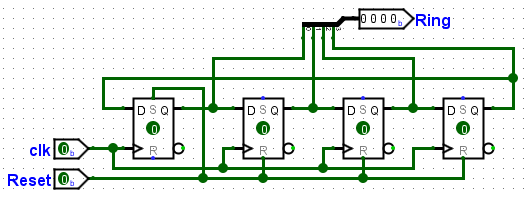
\includegraphics[width=\maxwidth{.95\linewidth}]{gfx/06-04}
	\caption{Synchronous Ring Counter}
	\label{fig:06-04}
\end{figure}

The following list describes the operation of the counter in Figure \ref{fig:06-04}:

\begin{description}
	\item [Reset is activated] \textit{U0} is set and \textit{U1}-\textit{U3} are reset so the counter is seeded with a single high bit to shift.
	
	%%%%%%%%%%%%%%%
	\item [Tick 1] \textit{Q0} \textdownarrow \: \textemdash \: \textit{Q1} \textuparrow
	
	%%%%%%%%%%%%%%%
	\item [Tick 2] \textit{Q1} \textdownarrow \: \textemdash \: \textit{Q2} \textuparrow
	
	%%%%%%%%%%%%%%%
	\item [Tick 3] \textit{Q2} \textdownarrow \: \textemdash \: \textit{Q3} \textuparrow
	
	%%%%%%%%%%%%%%%
	\item [Tick 4] \textit{Q3} \textdownarrow \: \textemdash \: \textit{Q1} \textuparrow
	
\end{description}

As the clock continues the counter would cycle through the binary values 0001 - 1000. The following table lists the \textit{ring} counter output as indicated by the \textit{Q} values at each tick listed above.

\begin{table}[H]
	\sffamily
	\newcommand{\head}[1]{\textcolor{white}{\textbf{#1}}}		
	\begin{center}
		\rowcolors{2}{gray!10}{white} % Color every other line a light gray
		\begin{tabular}{cc} 
			\rowcolor{black!75}
			\head{Tick} & \head{Output} \\
			Reset & 0001 \\
			1 & 0010 \\
			2 & 0100 \\
			3 & 1000 \\
			4 & 0001 \\
			5 & 0010 \\
			6 & 0100 \\
			7 & 1000 \\
			8 & 0001 
		\end{tabular}
	\end{center}
	\caption{Ring Counter Output}
	\label{tab0604}
\end{table}

\subsection{Synchronous Johnson Counter}

A Johnson Counter is similar to a ring counter in that a high bit value is shifted through the entire binary word. The difference is that the feedback loop comes from the \textit{Q'} output of the last stage rather than the \textit{Q} output. This type of counter is sometimes called a ``twisted tail'' counter since the \textit{Q'} output is fedback.

\begin{figure}[H]
	\centering
	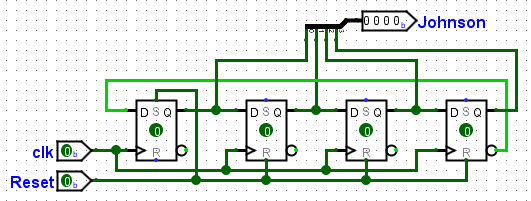
\includegraphics[width=\maxwidth{.95\linewidth}]{gfx/06-05}
	\caption{Synchronous Johnson Counter}
	\label{fig:06-05}
\end{figure}

The following list describes the operation of the counter in Figure \ref{fig:06-05}:

\begin{description}
	\item [Reset is activated] \textit{U0} is set and \textit{U1}-\textit{U3} are reset so the counter is seeded with a single high bit to shift.
	
	%%%%%%%%%%%%%%%
	\item [Tick 1] \textit{Q1} \textuparrow 
	
	%%%%%%%%%%%%%%%
	\item [Tick 2] \textit{Q2} \textuparrow
	
	%%%%%%%%%%%%%%%
	\item [Tick 3] \textit{Q3} \textuparrow 
	
	%%%%%%%%%%%%%%%
	\item [Tick 4] \textit{Q0} \textdownarrow

	%%%%%%%%%%%%%%%
	\item [Tick 5] \textit{Q1} \textdownarrow

	%%%%%%%%%%%%%%%
	\item [Tick 6] \textit{Q2} \textdownarrow
	
	%%%%%%%%%%%%%%%
	\item [Tick 7] \textit{Q3} \textdownarrow

	%%%%%%%%%%%%%%%
	\item [Tick 8] \textit{Q0} \textuparrow

\end{description}

As the clock continues the counter would cycle through the binary values 0000 - 1111. The following table lists the \textit{Johnson} counter output as indicated by the \textit{Q} values at each tick listed above.

\begin{table}[H]
	\sffamily
	\newcommand{\head}[1]{\textcolor{white}{\textbf{#1}}}		
	\begin{center}
		\rowcolors{2}{gray!10}{white} % Color every other line a light gray
		\begin{tabular}{cc} 
			\rowcolor{black!75}
			\head{Tick} & \head{Output} \\
			Reset & 0001 \\
			1 & 0011 \\
			2 & 0111 \\
			3 & 1111 \\
			4 & 1110 \\
			5 & 1100 \\
			6 & 1000 \\
			7 & 0000 \\
			8 & 0001 
		\end{tabular}
	\end{center}
	\caption{Johnson Counter Output}
	\label{tab0605}
\end{table}

\subsection{Main}

The \lstinline[columns=fixed]|main| circuit provides a human interface to try out each of the counters by dropping them in place of the \textit{Up} counter.

\begin{figure}[H]
	\centering
	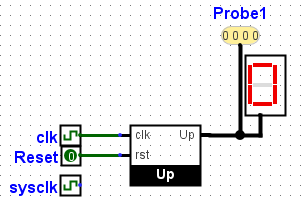
\includegraphics[width=\maxwidth{.95\linewidth}]{gfx/06-06}
	\caption{Main Circuit}
	\label{fig:06-06}
\end{figure}

Notice that there are two clocks in the \lstinline[columns=fixed]|main| circuit. \textit{Clk} is linked to the counter under test and needs no further explanation. \textit{Sysclk} is used by the \textit{Logisim-evolution} chronogram as described in the next section of this document.

\subsection{Chronogram}

\textit{Logisim-evolution} can generate a timing diagram, called a \textit{chronogram}, for a sequential circuit. That is a representation of the various signals in a circuit and how those signals change over time. Figure \ref{fig:06-07} is the timing diagram for an Up counter.

\begin{figure}[H]
	\centering
	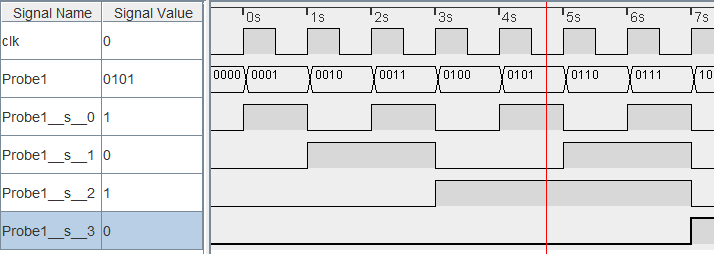
\includegraphics[width=\maxwidth{.95\linewidth}]{gfx/06-07}
	\caption{Timing Diagram for Up Counter}
	\label{fig:06-07}
\end{figure}

At the top of Figure \ref{fig:06-07} is a scale that indicates the number of seconds that the counter has been operating. The first trace is the input clk signal. The clock goes high at the start of each second and then goes low at the half-second mark. Under the clock is the ``Probe1'' signal. Because that is a four-bit number \textit{Logisim-evolution} displays the number, but under that number is a breakout of the four bits that make up that number. Thus, at time zero ``Probe1'' is 0001 and ``Probe1\_s\_0'' (that stands for ``Probe 1, Signal 0'') is high while the other bits are low. The \textit{Logisim-evolution} \textit{chronogram} includes a cursor indicated by a red line (found just before the five second tick in Figure \ref{fig:06-07}) that can be placed anywhere along the diagram. The cursor sets the values of each signal in the area on the left edge of the diagram, so the cursor in Figure \ref{fig:06-07} is pointing to a spot where the \textit{clk} is low, \textit{Probe1} is at 0101, and so forth.

Follow the next steps to use the chronogram. Notes: the chronogram will only check subcircuits that are found on the  \lstinline[columns=fixed]|main| subcircuit. Therefore, in order to create a timing diagram all subcircuits need to be combined on \lstinline[columns=fixed]|main|. The labs completed in this manual have been designed to use the \lstinline[columns=fixed]|main| subcircuit as the human interface so the chronogram feature will work well with these circuits. 

\begin{enumerate}
	\item In the \lstinline[columns=fixed]|main| subcircuit, add a ``sampling clock'' labeled \textit{sysclk} (this name is important, do not change it to something else). The sampling clock is only used by the \textit{chronogram} and will not show up in the timing diagram. It should not be connected to any other components and can be placed anywhere on \lstinline[columns=fixed]|main|. Set the properties for \textit{sysclk} to a 1 Tick high duration and a 1 Tick low duration (this is the default). 
	\item Add a circuit master clock labeled \textit{clk}. This is the clock that will be used to trigger all components in the circuit. Set the properties for \textit{clk} to a 4 Tick high duration and a 4 Tick low duration.
	\item Set \textsc{Simulate -> Tick Frequency} to 4 Hertz. This will simulate a clock that ticks once per second, as in Figure \ref{fig:06-07}. While the actual tick frequency can be changed later to ``speed up'' the circuit, a one-second tick is useful for learning how the \textit{chronogram} works.
	\item Click \textsc{Simulate -> Chronogram} to set up the \textit{chronogram}. Figure \ref{fig:06-08} illustrates the initial setup screen for the \textit{chronogram}.

	\begin{figure}[H]
		\centering
		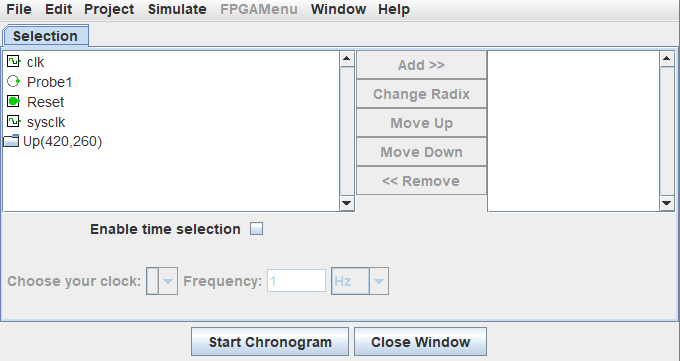
\includegraphics[width=\maxwidth{.95\linewidth}]{gfx/06-08}
		\caption{Set Up Chronogram}
		\label{fig:06-08}
	\end{figure}

	\item Click \textit{sysclk} in the left panel and then click \textit{Add >>} to add that signal to the \textit{chronogram}. The ``-2'' following the \textit{sysclk} name in the right panel indicates that it is a binary signal. NOTE: \textit{sysclk} must be added to the \textit{chronogram} or it will not sample the circuit; however, the \textit{sysclk} signal will not actually show up in the timing diagram. It is probably best to add the \textit{sysclk} signal first so it is not overlooked.
	\item Click \textit{clk} in the left panel and then click \textit{Add >>} to add that signal to the \textit{chronogram}.
	\item Click \textit{Probe1} in the left panel and then click \textit{Add >>} to add that signal to the \textit{chronogram}.
	\item Click ``Enable time selection'' and chose \textit{clk} as the clock with a frequency of 1 Hertz.
	\item The \textit{chronogram} setup should look like Figure \ref{fig:06-09}.
	
	\begin{figure}[H]
		\centering
		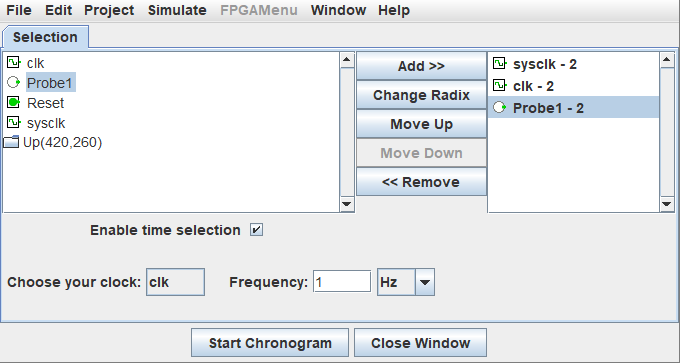
\includegraphics[width=\maxwidth{.95\linewidth}]{gfx/06-09}
		\caption{Chronogram Ready}
		\label{fig:06-09}
	\end{figure}

	\item Click \textit{Start Chronogram} and the screen illustrated in Figure \ref{fig:06-10} pops up.
	
	\begin{figure}[H]
		\centering
		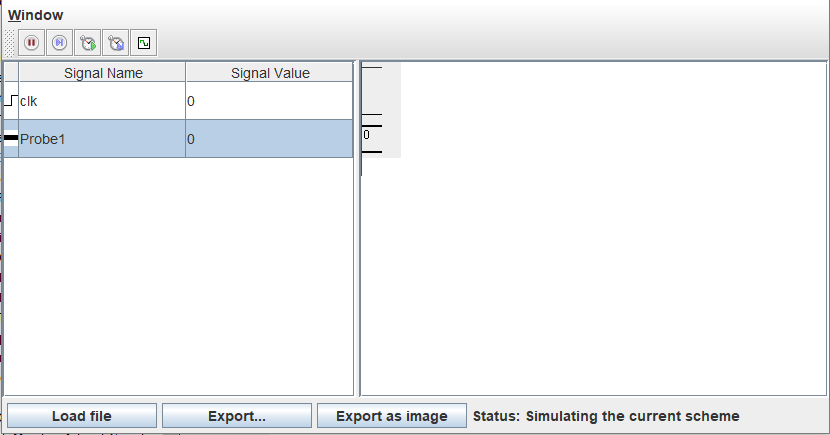
\includegraphics[width=\maxwidth{.95\linewidth}]{gfx/06-10}
		\caption{Chronogram Starting}
		\label{fig:06-10}
	\end{figure}
	
	\item Right-click on the \textit{Probe1} signal and set the format for binary. The format can be set for any radix but to match this lab binary numbers should be specified.
	\item Right-click on the \textit{Probe1} signal and enable \textit{Expand} to see all four signals that create \textit{Probe1}.
	\item At this point, the chronogram should look like Figure \ref{fig:06-11}.
	
	\begin{figure}[H]
		\centering
		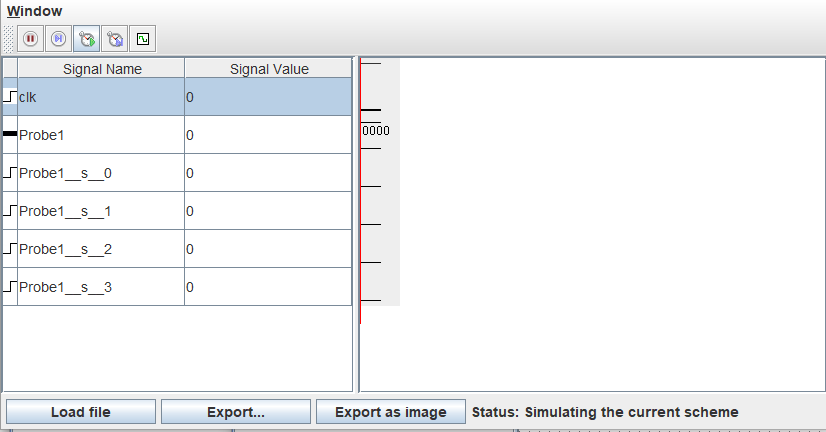
\includegraphics[width=\maxwidth{.95\linewidth}]{gfx/06-11}
		\caption{Chronogram At Zero Time}
		\label{fig:06-11}
	\end{figure}
	
	\item The \textit{chronogram} has five buttons that control the simulator.
	
	\begin{figure}[H]
		\centering
		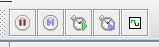
\includegraphics[width=\maxwidth{.95\linewidth}]{gfx/06-12}
		\caption{Chronogram Controls}
		\label{fig:06-12}
	\end{figure}
	
	\begin{itemize}
		\item Button One: Start/Stop the simulation.
		\item Button Two: Simulate one step.
		\item Button Three: Start/Stop \textit{sysclk}. This will ``turn on'' the chronogram and begin creating a timing diagram.
		\item Button Four: Step one \textit{sysclk} tick. This will tick the \textit{sysclk} one time. Since this lab set up the \textit{sysclk} for four ticks per second this button would need to be clicked four times to extend the timing diagram one second.
		\item Button Five: Step one \textit{clk} tick. This extends the timing diagram by one complete clock tick, or one second in this circuit.
	\end{itemize}
	
	\item Click button three to start the \textit{chronogram} and watch the timing diagram unfold. After a few seconds click that button a second time to stop the \textit{chronogram}.
	
	\item The following can be done once the timing diagram is complete.
	
	\begin{itemize}
		\item Click on the timing diagram to set the cursor (indicated by a red line). Once the cursor is set the values for each signal at the cursor's location are printed next to the signal's label on the left edge of the timing diagram.
		\item Hover the mouse over the timing diagram and roll the mouse wheel to zoom the timing diagram appearance.
		\item Click ``Export'' to save the timing diagram signal levels in a text file. That file can later be loaded to reevaluate the timing diagram.
		\item Click ``Export as image'' to save the timing diagram as a PNG file.
	\end{itemize}
	
\end{enumerate}

\section{Challenge}

This lab includes several different timers. Place all of them on a single subcircuit named \lstinline[columns=fixed]|Universal| that includes an output mux so a user can select the type of counter output desired. Place the \lstinline[columns=fixed]|Universal| circuit on \lstinline[columns=fixed]|main| and wire appropriate inputs and outputs.

Set up the chronogram for the ring counter and create a ten-second timing diagram for that counter. Save the timing diagram as a PNG image named ``RingCounter.''

\section{Deliverable}

To receive a grade for this lab, complete the Challenge. Be sure the standard identifying information is at the top left of the \lstinline{main} circuit: 

\bigskip
% The minipage environment keeps the three lines together - no page break.
\begin{minipage}{\linewidth}
	\begin{verbatim}
	George Self
	Lab 06: Counters
	March 17, 2018
	\end{verbatim}
\end{minipage}
\bigskip

Save the circuit with this name: \textit{Lab07\_counter} and submit that along with \textit{RingCounter.PNG} for grading.

